\documentclass[a4 paper]{article}
% Set target color model to RGB
\usepackage[inner=2.0cm,outer=2.0cm,top=2.5cm,bottom=2.5cm]{geometry}
\usepackage{setspace}
\usepackage[rgb]{xcolor}
\usepackage{verbatim}
\usepackage{subcaption}
\usepackage{amsgen,amsmath,amstext,amsbsy,amsopn,tikz,amssymb}
\usepackage{fancyhdr}
\usepackage[colorlinks=true, urlcolor=blue,  linkcolor=blue, citecolor=blue]{hyperref}
\usepackage[colorinlistoftodos]{todonotes}
\usepackage{rotating}
\usepackage{enumitem}
\usepackage{float}

%\usetikzlibrary{through,backgrounds}
\hypersetup{%
pdfauthor={Aishik Mandal},%
pdftitle={Homework 0},%
pdfkeywords={Tikz,latex,bootstrap,uncertaintes},%
pdfcreator={PDFLaTeX},%
pdfproducer={PDFLaTeX},%
}
%\usetikzlibrary{shadows}
% \usepackage[francais]{babel}
\usepackage{booktabs}
% \input{macros.tex}

\newcommand{\ra}[1]{\renewcommand{\arraystretch}{#1}}

\newtheorem{thm}{Theorem}[section]
\newtheorem{prop}[thm]{Proposition}
\newtheorem{lem}[thm]{Lemma}
\newtheorem{cor}[thm]{Corollary}
\newtheorem{defn}[thm]{Definition}
\newtheorem{rem}[thm]{Remark}
\numberwithin{equation}{section}

\newcommand{\homework}[5]{
   \pagestyle{myheadings}
   \thispagestyle{plain}
   \newpage
   \setcounter{page}{1}
   \noindent
   \begin{center}
   \framebox{
      \vbox{\vspace{2mm}
    \hbox to 6.28in { {\bf Ethics for NLP: SS 2024 \hfill {\small (#2)}} }
       \vspace{6mm}
       \hbox to 6.28in { {\Large \hfill #1  \hfill} }
       \vspace{6mm}
       \hbox to 6.28in {  {\it Name: {\rm #3}
        %NetID: {\rm #4} 
        \hfill Matriculation No.: {\rm #5}} }
      \vspace{2mm}}
   }
   \end{center}
   \markboth{#5 -- #1}{#5 -- #1}
   \vspace*{4mm}
}

\newcommand{\problem}[2]{~\\\fbox{\textbf{Problem #1}}\newline\newline}
\newcommand{\subproblem}[1]{~\newline\textbf{(#1)}}
\newcommand{\D}{\mathcal{D}}
\newcommand{\Hy}{\mathcal{H}}
\newcommand{\VS}{\textrm{VS}}

\newcommand{\bbF}{\mathbb{F}}
\newcommand{\bbX}{\mathbb{X}}
\newcommand{\bI}{\mathbf{I}}
\newcommand{\bX}{\mathbf{X}}
\newcommand{\bY}{\mathbf{Y}}
\newcommand{\bepsilon}{\boldsymbol{\epsilon}}
\newcommand{\balpha}{\boldsymbol{\alpha}}
\newcommand{\bbeta}{\boldsymbol{\beta}}
\newcommand{\0}{\mathbf{0}}
\newcommand{\code}[1]{\texttt{#1}}


\begin{document}

\homework{Homework 0}{Due: 08 May 2024, 11:59pm}{Julian Steiner}{}{2669944}

%Read all the instructions carefully before you start working on the assignment, and before you make a submission.

\problem{1}

\subproblem{1.4}

In Figure \ref{fig:conf_matrix_val} the confusion matrix calculated on the validation set is shown. In Figure \ref{fig:conf_matrix_test} the confusion matrix calculated on the test set is shown. The classifier reached 76\% accuracy on the validation set and on the test set even 93\%. But the accuracy metric is misleading here. The classifier classifies the texts with a higher probability with label 4, i.e. a rating of 5.  Despite incorrect predictions, a high accuracy can be reached. If the dataset, on which the accuracy are calculated, contains many examples with label 4 and the classifier predicts label 4 with a higher probability, many will still be predicted correctly. We can see this from the calculated confusion matrix on the test set. In total, this dataset contains 250 label 4 samples, which are all predicted correctly. On the other hand, the data set contains only 20 samples with other labels, most of which are classified also as with label 4. Due to the many label 4 samples in the test set that are correctly predicted, this leads to a high accuracy.

\begin{center}
    \begin{figure}[H]
        \centering
        \begin{subfigure}[b]{0.49\textwidth}
            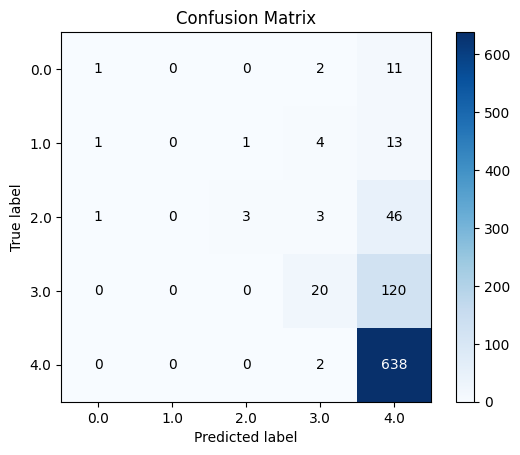
\includegraphics[width=\textwidth]{confusion_matrix_val_set}
            \caption{Confusion matrix on validation set.}
            \label{fig:conf_matrix_val}
        \end{subfigure}
        \hfill
        \begin{subfigure}[b]{0.49\textwidth}
            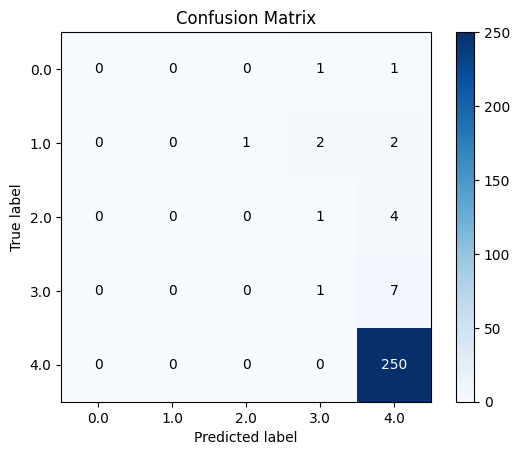
\includegraphics[width=\textwidth]{confusion_matrix_test_set}
            \caption{Confusion matrix on test set.}
            \label{fig:conf_matrix_test}
        \end{subfigure}
        \caption{Confusion matrix on different datasets.}
        \label{fig:confusion_matrix}
    \end{figure}
\end{center}

One reason may be that the training, validation and test data predominantly contain examples with a rating of 5, i.e. label 4. The distribution of the ratings of each dataset is shown in Figure \ref{fig:dataset_distributions}. Note: This distributions don't show the preprocessed data and also includes empty texts, which are filtered out for training the model. Another note: Rating is not the label. The label of a respective rating is always the rating minus one. In addition, there can be many other reasons, i.e. the model architecture.

\begin{center}
    \begin{figure}[H]
        \centering
        \begin{subfigure}[b]{0.49\textwidth}
            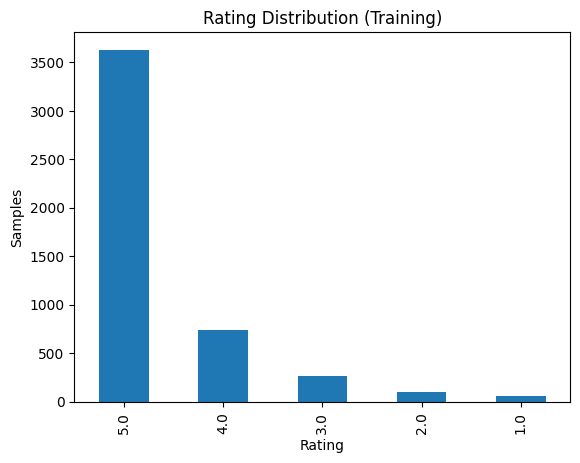
\includegraphics[width=\textwidth]{dist_training}
            \caption{Rating distribution of training set.}
            \label{fig:dist_training}
        \end{subfigure}
        \hfill
        \begin{subfigure}[b]{0.49\textwidth}
            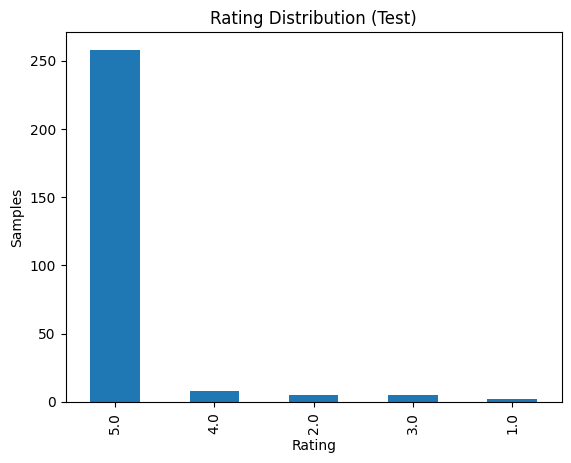
\includegraphics[width=\textwidth]{dist_test}
            \caption{Rating distribution of test set.}
            \label{fig:dist_test}
        \end{subfigure}
        \hfill
        \begin{subfigure}[b]{0.49\textwidth}
            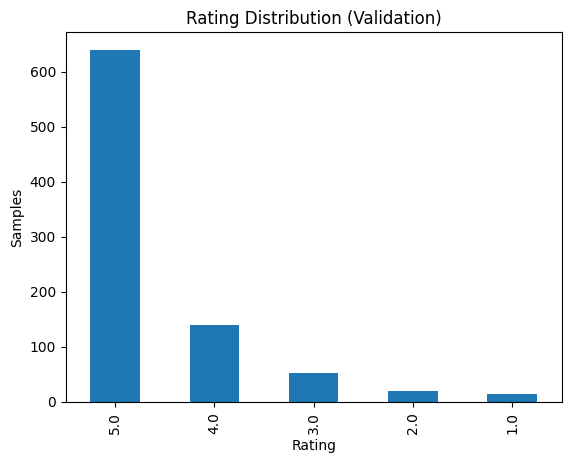
\includegraphics[width=\textwidth]{dist_validation}
            \caption{Rating distribution of validation set.}
            \label{fig:dist_validation}
        \end{subfigure}
        \caption{Rating distribution of different datasets.}
        \label{fig:dataset_distributions}
    \end{figure}
\end{center}

\problem{2}

\subproblem{2.1}

\begin{itemize}
 \item (1): Benefit from such a classifier would the teacher or the professor. He or she would no longer have to evaluate the essays or use the classifier as support for grading the essays. But students could also benefit. Students could get immediate feedback on their submission without having to wait for the long correction period.
 \item (2): The students could be harmed by such a system. For example, incorrect grading could unfairly punish or reward students. In addition the teachers could also be harmed. The teacher could rely too heavily on the classifier and may overlook important things in the student essays.
 \item (3): The data is not representative. The data is only from one course of one year. The diversity in the data set could be missing. For example, from other courses, other universities and also from several years.
 \item (4): Ethical concerns regarding data collection may arise from the explicit consent of the participants with whom the classifier was trained. Have the students consented to the use of their essays for the task of training a classifier?
 \item (5): Neural networks are black boxes, so to speak. It is not possible to understand exactly what criteria the model used to arrive at its prediction. Therefore, I would say that neural networks, as long as they do not make their prediction comprehensible, are not a suitable modeling approach for the task. On the other hand, neural networks are the best approach for modeling NLP at the moment. Of course with different architectures than we used in the exercise. This raises the question of whether it is generally a good idea to develop models for such purposes.
 \item (6): A possible dual use for such a classifier could be, for example, that the classifier classifies the essay according to how closely the opinion of the essay matches that of the teacher. This could limit the diversity of opinion within courses and lead to unfair and subjective assessments.
\end{itemize}

\subproblem{2.2}

I think, there are several issues with project A that need to be clarified by the ethics board. First, in the research project idea is mentioned that the tool tries "to find other papers related to each sentence - even if they are not cited in the main paper". How can it be ensured that for the respective sentence, it is a correct classification of the found paper, even if it was not cited. In the case of misclassification, the author of the paper could be falsely suspected of plagiarism because he or she did not cite the found paper. As a result, the author could be falsely harmed. Secondly, are the researchers allowed to use the publicly accessible research papers for their study? Thirdly, the researcher "will record the participants using the tool via screen recording, and analyize the recordings to improve the usability of the tool". Is this collection of data the absolute necessary minimum for this study?

On the one hand, the participants in Project B are lied to. The participants are informed that the study is being conducted by the psychology department, although it is being conducted by computer science department. In addition, the participants do not know that they are interacting with a chatbot. The board must clarify whether these lies are necessary to achieve the objectives of the research. Another point that should be examined by the ethics board is whether the participant could be harmed if the chatbot is placed on the "politness" level rude.

\end{document}
